\documentclass{standalone}
\pagestyle{empty}
\usepackage{tikz}
\usetikzlibrary{arrows.meta,bending}

\begin{document}
\noindent
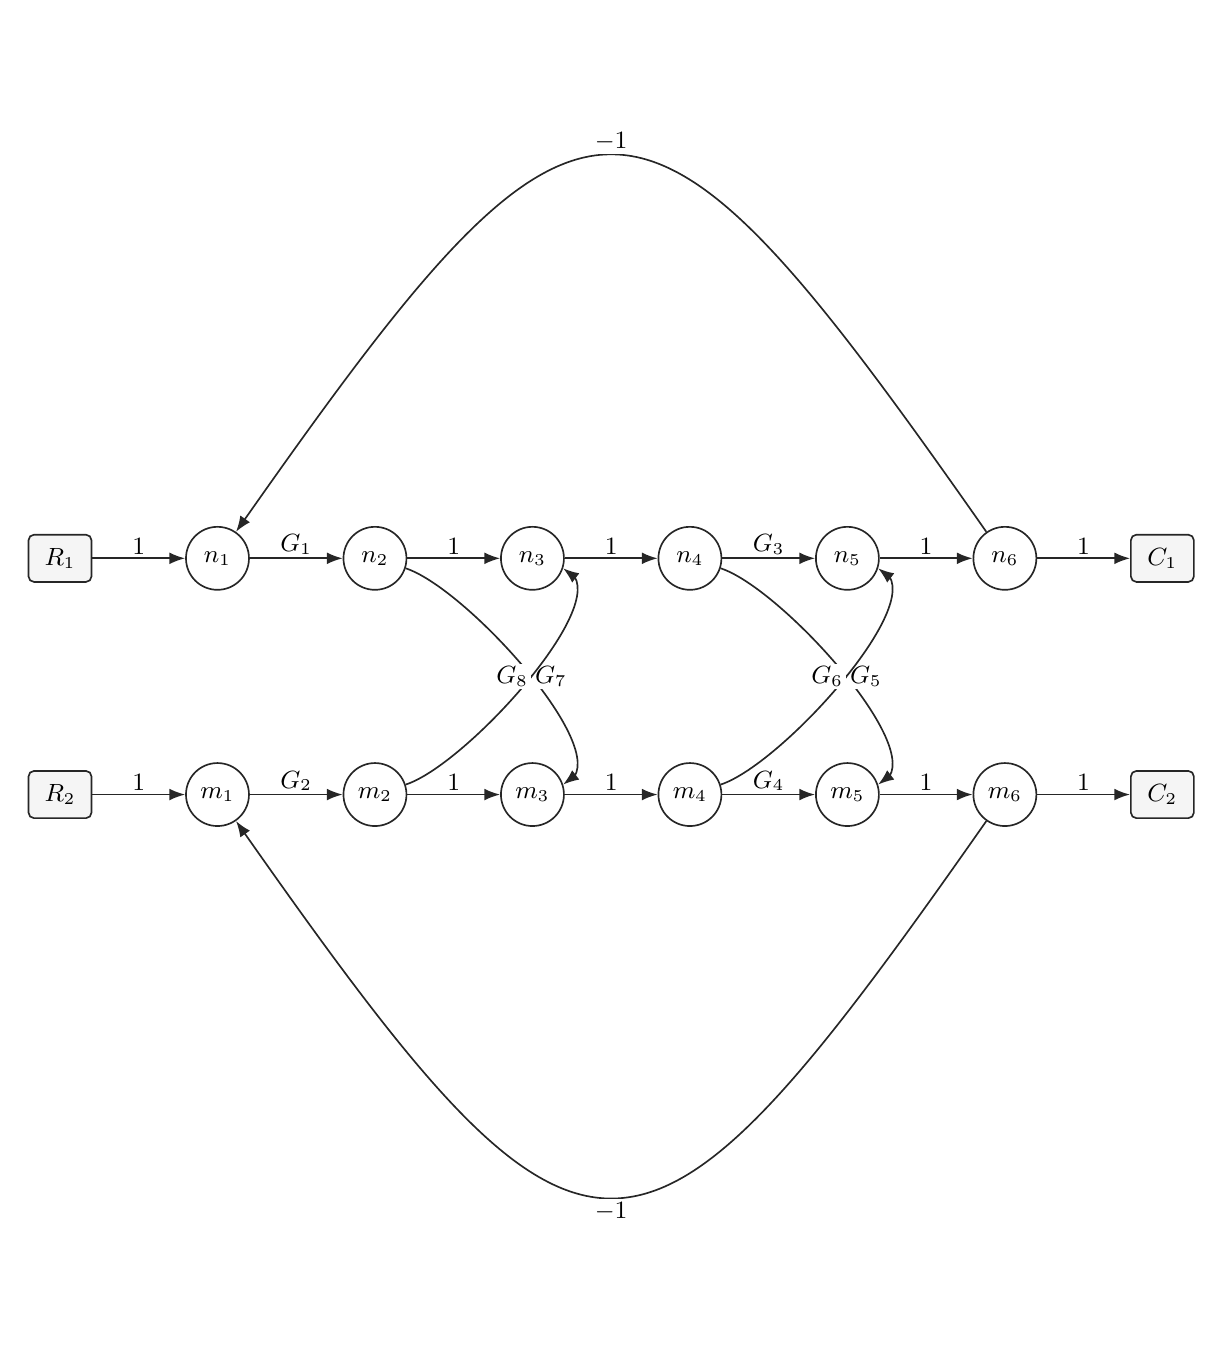
\begin{tikzpicture}[
  >=Latex,
  ->,
  semithick,
  every node/.style={font=\small},
  signal node/.style={circle,draw,minimum size=8mm,inner sep=1pt,fill=white},
  io node/.style={rectangle,rounded corners=2pt,draw,minimum width=8mm,minimum height=6mm,inner sep=2pt,fill=gray!8},
  every path/.style={draw=black!85},
  edge label/.style={fill=white,inner sep=1pt,text=black},
]
\node[signal node] (n1) at (2.0,3.0) {$n_1$};
\node[signal node] (n2) at (4.0,3.0) {$n_2$};
\node[signal node] (n3) at (6.0,3.0) {$n_3$};
\node[signal node] (n4) at (8.0,3.0) {$n_4$};
\node[signal node] (n5) at (10.0,3.0) {$n_5$};
\node[signal node] (n6) at (12.0,3.0) {$n_6$};
\node[io node] (R1) at (0.0,3.0) {$R_1$};
\node[io node] (C1) at (14.0,3.0) {$C_1$};
\node[signal node] (m1) at (2.0,0.0) {$m_1$};
\node[signal node] (m2) at (4.0,0.0) {$m_2$};
\node[signal node] (m3) at (6.0,0.0) {$m_3$};
\node[signal node] (m4) at (8.0,0.0) {$m_4$};
\node[signal node] (m5) at (10.0,0.0) {$m_5$};
\node[signal node] (m6) at (12.0,0.0) {$m_6$};
\node[io node] (R2) at (0.0,0.0) {$R_2$};
\node[io node] (C2) at (14.0,0.0) {$C_2$};
\draw (R1) -- node[edge label,midway,above] {$1$} (n1);
\draw (n1) -- node[edge label,midway,above] {$G_1$} (n2);
\draw (n2) -- node[edge label,midway,above] {$1$} (n3);
\draw (n3) -- node[edge label,midway,above] {$1$} (n4);
\draw (n4) -- node[edge label,midway,above] {$G_3$} (n5);
\draw (n5) -- node[edge label,midway,above] {$1$} (n6);
\draw (n6) -- node[edge label,midway,above] {$1$} (C1);
\draw (R2) -- node[edge label,midway,above] {$1$} (m1);
\draw (m1) -- node[edge label,midway,above] {$G_2$} (m2);
\draw (m2) -- node[edge label,midway,above] {$1$} (m3);
\draw (m3) -- node[edge label,midway,above] {$1$} (m4);
\draw (m4) -- node[edge label,midway,above] {$G_4$} (m5);
\draw (m5) -- node[edge label,midway,above] {$1$} (m6);
\draw (m6) -- node[edge label,midway,above] {$1$} (C2);
\draw (n6) to[out=125,in=55,looseness=2.10] node[edge label,midway,above] {$-1$} (n1);
\draw (m6) to[out=-125,in=-55,looseness=2.10] node[edge label,midway,below] {$-1$} (m1);
\draw (n2) to[out=-18,in=18,looseness=0.63] node[edge label,midway,right] {$G_7$} (m3);
\draw (m2) to[out=18,in=-18,looseness=0.63] node[edge label,midway,left] {$G_8$} (n3);
\draw (n4) to[out=-18,in=18,looseness=0.63] node[edge label,midway,right] {$G_5$} (m5);
\draw (m4) to[out=18,in=-18,looseness=0.63] node[edge label,midway,left] {$G_6$} (n5);
\end{tikzpicture}
\end{document}
